% Compact PGFPlots panel for sampled surface11 BSC bit-scale decomposition.
% Requires \usepackage{pgfplots} and \pgfplotsset{compat=1.18}.
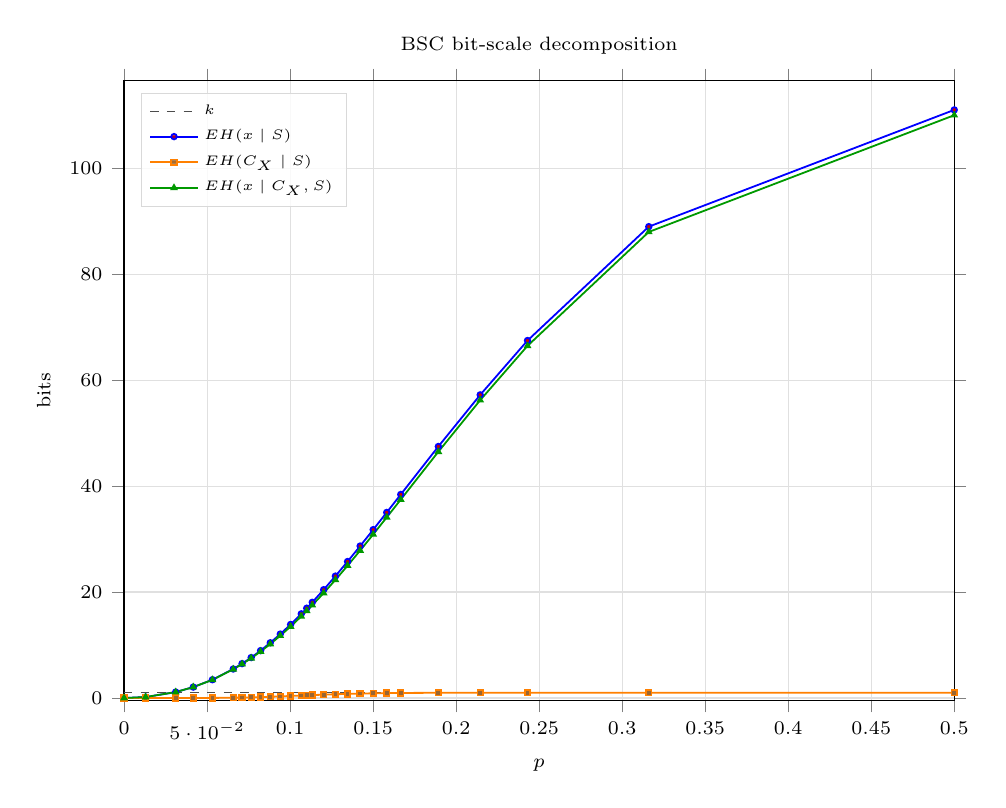
\begin{tikzpicture}
\begin{axis}[
  name=Surface11BSCBitScaleAxis,
  width=\linewidth,
  height=0.78\linewidth,
  title={BSC bit-scale decomposition},
  title style={font=\scriptsize},
  xlabel={$p$},
  ylabel={bits},
  xmin=0, xmax=0.5,
  ymin=-0.5, ymax=116.55,
  grid=both,
  major grid style={black!12},
  minor grid style={black!6},
  tick align=outside,
  tick label style={font=\scriptsize},
  label style={font=\scriptsize},
  legend cell align={left},
  legend style={draw=black!15, fill=white, fill opacity=0.82, text opacity=1, at={(0.02,0.98)}, anchor=north west, font=\tiny},
]
\addplot[black!70, dashed, line width=0.55pt] coordinates {(0,1) (0.5,1)};
\addlegendentry{$k$}
\addplot+[color=blue, mark=*, mark size=1.0pt, line width=0.65pt]
coordinates {(0,0) (0.0129868620555,0.181054493335) (0.0311244603048,1.1227635552) (0.0416926902737,2.06191337851) (0.0532390407768,3.45157333133) (0.0657867063546,5.47786643398) (0.0710958755299,6.49372028352) (0.0765765344037,7.63453655645) (0.0822333323659,8.94027725026) (0.0880715694979,10.4241416696) (0.0940972433461,12.0699271602) (0.100317108961,13.8726766994) (0.106738753821,15.8805917291) (0.110027864438,16.946951122) (0.113370689941,18.0648188099) (0.120222466333,20.440050262) (0.127304805976,23.0112445174) (0.134629772869,25.7577379629) (0.142210976498,28.6858085582) (0.150063823499,31.7728180307) (0.158205829694,35.0242794846) (0.166657010397,38.4147966319) (0.189297705371,47.4725433676) (0.21450174486,57.2145528255) (0.243003853809,67.468384113) (0.316019346324,88.9612825378) (0.5,111)};
\addlegendentry{$\mathbb{E}H(x\mid S)$}
\addplot+[color=orange, mark=square*, mark size=1.0pt, line width=0.65pt]
coordinates {(0,0) (0.0129868620555,2.61675620426e-08) (0.0311244603048,0.000217887541169) (0.0416926902737,0.00393091101468) (0.0532390407768,0.0185000665939) (0.0657867063546,0.0583636541452) (0.0710958755299,0.0865901691606) (0.0765765344037,0.124791305066) (0.0822333323659,0.173561297785) (0.0880715694979,0.233556072119) (0.0940972433461,0.306681005333) (0.100317108961,0.383186610519) (0.106738753821,0.467128119501) (0.110027864438,0.508581080162) (0.113370689941,0.549632805412) (0.120222466333,0.63412093105) (0.127304805976,0.711217092285) (0.134629772869,0.781094381439) (0.142210976498,0.840909315233) (0.150063823499,0.888316492504) (0.158205829694,0.926635123075) (0.166657010397,0.953888696697) (0.189297705371,0.989137245186) (0.21450174486,0.998535750807) (0.243003853809,0.999947023908) (0.316019346324,1.00000072526) (0.5,1)};
\addlegendentry{$\mathbb{E}H(C_X\mid S)$}
\addplot+[color=green!60!black, mark=triangle*, mark size=1.0pt, line width=0.65pt]
coordinates {(0,0) (0.0129868620555,0.181054467167) (0.0311244603048,1.12254566766) (0.0416926902737,2.0579824675) (0.0532390407768,3.43307326474) (0.0657867063546,5.41950277983) (0.0710958755299,6.40713011436) (0.0765765344037,7.50974525138) (0.0822333323659,8.76671595247) (0.0880715694979,10.1905855975) (0.0940972433461,11.7632461549) (0.100317108961,13.4894900888) (0.106738753821,15.4134636096) (0.110027864438,16.4383700419) (0.113370689941,17.5151860045) (0.120222466333,19.805929331) (0.127304805976,22.3000274251) (0.134629772869,24.9766435815) (0.142210976498,27.844899243) (0.150063823499,30.8845015382) (0.158205829694,34.0976443615) (0.166657010397,37.4609079352) (0.189297705371,46.4834061224) (0.21450174486,56.2160170747) (0.243003853809,66.4684370891) (0.316019346324,87.9612818125) (0.5,110)};
\addlegendentry{$\mathbb{E}H(x\mid C_X,S)$}
\end{axis}
\end{tikzpicture}
